
\section{Background and Related Work}
\subsection{The PageRank Algorithm}
% Describe how PageRank works: power iteration, damping factor, convergence.

\subsubsection{Origins and Motivation}
\subsubsection{Graph Representation and the Transition Matrix}
\subsubsection{The Random Surfer Model and Damping Factor}
\subsubsection{Mathematical Definition of PageRank}
\subsubsection{Power Iteration and Convergence}
\subsubsection{Complexity and other Variants (Personalized PageRank)}


PageRank is an algorithm that was originally introduced to measure the relevance of websites on the World Wide Web. The more websites that link to a website, the higher its rank. Created by Google founders Larry Page and Sergey Brin, it was designed to optimize the search engine \cite{page_pagerank_1999}.
The algorithm is based on a graph where each node represents a website on the internet, and each edge represents a hyperlink on a website.
\begin{figure}[ht]
    \centering
    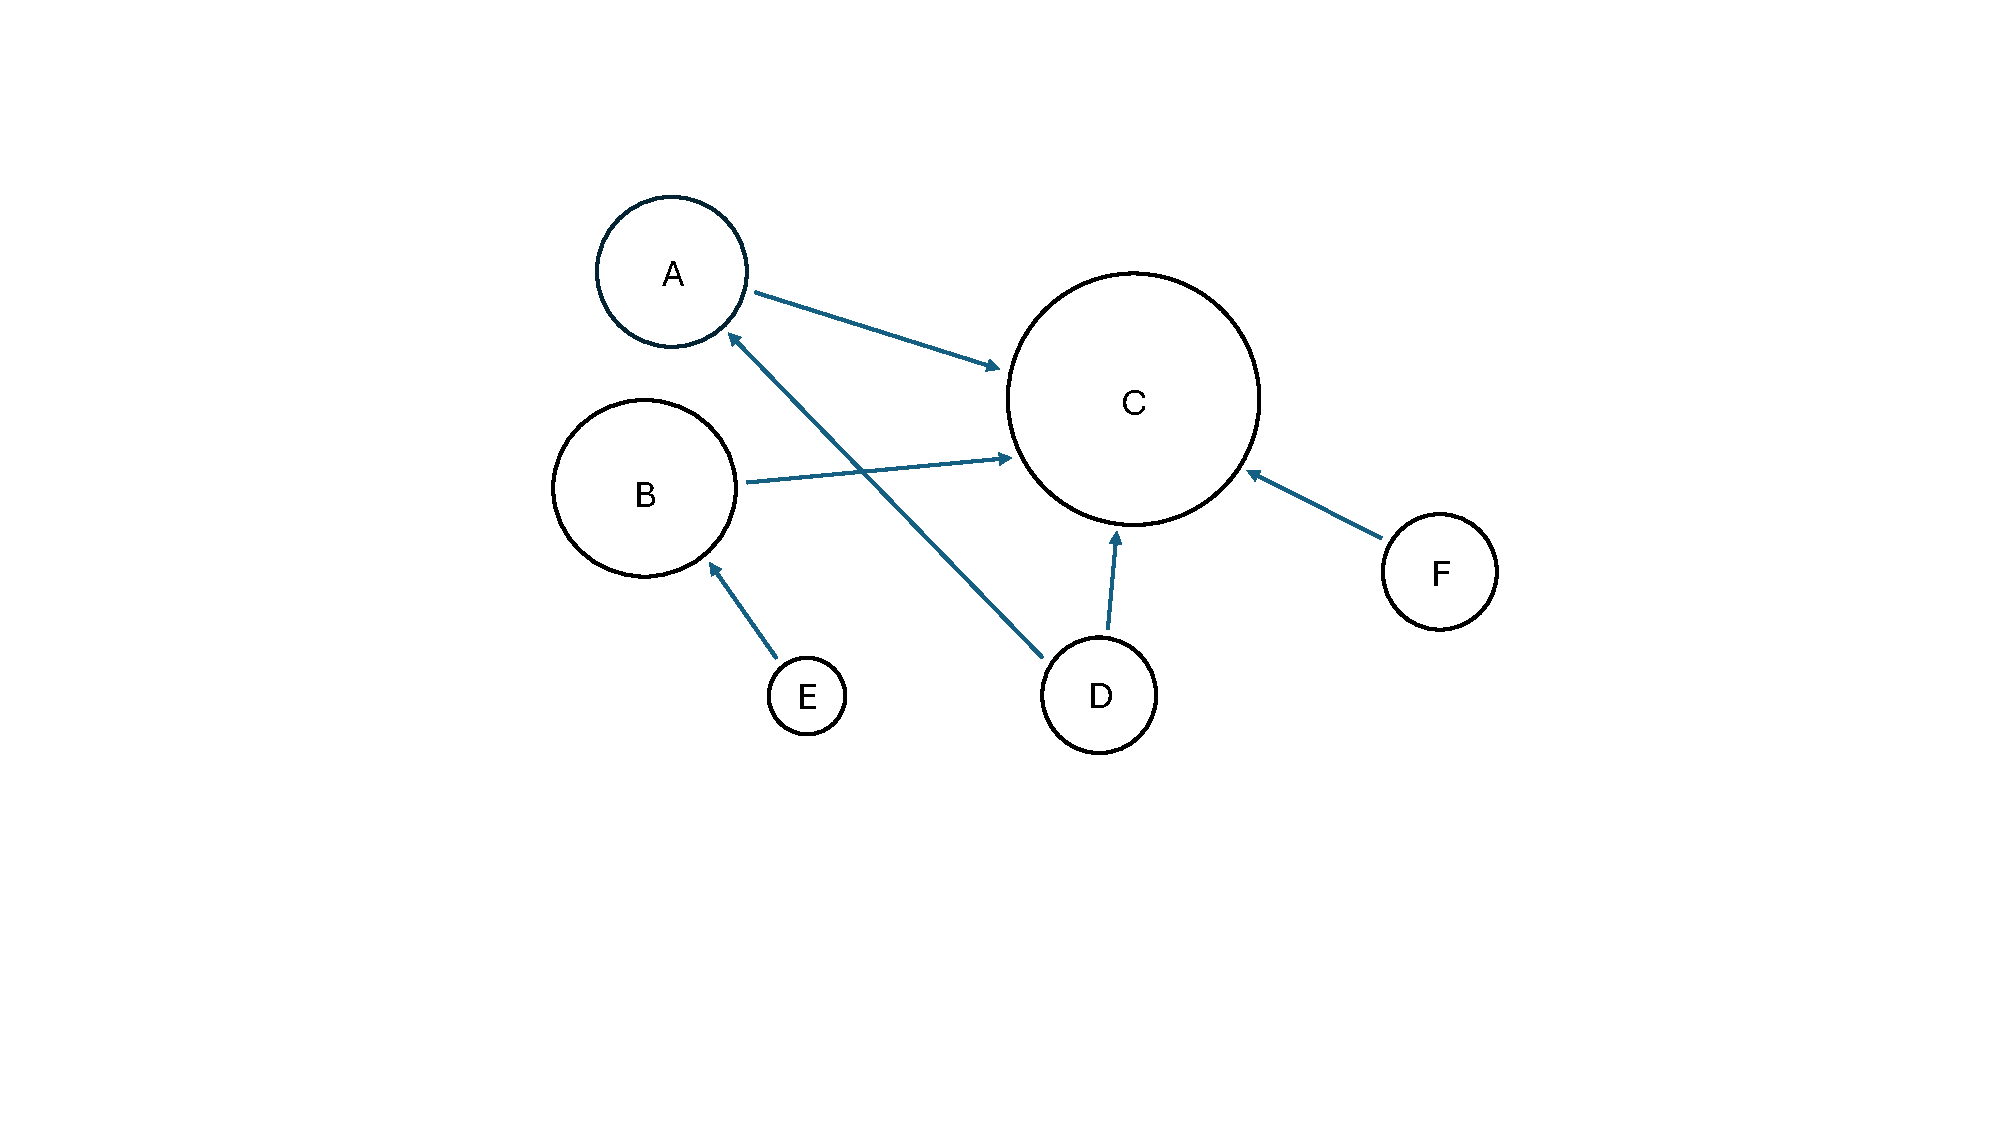
\includegraphics[width=0.7\linewidth]{images/PageRank Graph.pdf}
    \caption{PageRank Graph}
    \label{fig:pagerank-toy}
\end{figure}

To calculate PageRank values, a transition matrix is constructed. Each row of the matrix represents a state or website and contains the probabilities of moving from one node to another. Figure 1 shows that D has two outgoing edges, so the probability of moving from D to another node is $0.5$. The transition matrix describes the behavior of a "random surfer". The random surfer model describes the probability of a random user visiting a website. Finding the PageRank values is a Markov chain process, and its stationary distribution is the PageRank vector. Additionally, to model realistic user behavior, a damping factor is introduced, which is commonly set to 0.85. That means with probability $\alpha$, a random surfer clicks on an outgoing hyperlink on the current website and with probability $1-\alpha$ the surfer "teleports" to a random website in the graph. This characteristic is necessary for PageRank because web graphs may contain dangling nodes, disconnected parts, or cycles. Thus, the damping factor ensures that the Markov chain is irreducible and aperiodic, guaranteeing convergence to a unique stationary distribution \cite{langville_googles_2012}. 
The PageRank algorithm is commonly defined as follows \cite{chebolu_pagerank_2008}:
\begin{equation}
    \pi_v = \frac{1-\alpha}{n}+c\sum_{u\in N^-(v)}\frac{\pi_u}{d^+(u)} 
\end{equation} 
where: 
\begin{itemize}
    \item $\pi_v$ is the PageRank of the node $v$
    \item $\alpha$ is the damping factor
    \item $n$ is the total number of nodes in the graph
    \item $N^-(v)$ is the set of ingoing edges of $v$
    \item $d^+(u)$ is the out degree of $u$
\end{itemize} 
% talk about tolerance and convergence
The calculation of PageRank follows the power iteration method, a technique to finding the dominant eigenvalue. The iterative process is defined as follows
\begin{enumerate}
    \item Define the initial vector 
    \begin{equation}
        \pi^{(0)}=\frac{1}{n}e
    \end{equation}
    \item At each iteration apply the update rule, where $S$ is the transition matrix and $e$ is the all-ones vector
    \begin{equation}
        \pi^{(k+1)} = \alpha S^T+ \frac{(1-\alpha)}{n}e
    \end{equation}
    \item Continue until the difference between iterations is less than a tolerance $\epsilon$
    \begin{equation}
        ||\pi^{(k+1)}-\pi^{(k)}||_1<\epsilon \quad \text{\cite{langville_googles_2012}\cite{page_pagerank_1999}}
    \end{equation}
    
\end{enumerate}
Then $\pi$ satisfies 
\begin{equation}
    \pi=G^T\pi, \quad \text{where $G=\alpha S +\frac{1-\alpha}{n}ee^T$}
\end{equation}
and $\pi$ is a stationary probability distribution, the unique PageRank vector.
Each entry in the PageRank vector represents the probability that a random surfer will land on a particular node. The power iteration method has a time complexity of $O(m)$ per iteration, where $m$ is the the number of edges. Thus, the total complexity is $O(m\cdot k)$. The number of iterations, $k$, depends on the damping factor, $\alpha$, and the tolerance ,$\epsilon$. After the original PageRank algorithm was introduced, many more variants were developed, such as Personalized PageRank (PPR) \cite{park_survey_2019}.
In this version, teleportation is not uniformly distributed across all nodes. Instead, the random surfer only jumps to a specific set of nodes called  "restarting nodes". The resulting PageRank vector measures how close or relevant each node is to the restarting nodes in the set \cite{priyanta_social_2019}. 

 
\subsection{Challenges in Large-Scale Graph Processing}

\subsubsection{Growth of Graph Data}
\subsubsection{Memory Bottlenecks of PageRank}
\subsubsection{Computational Complexity and Iterations}
\subsubsection{Limits of Single-Machine Processing}
\subsubsection{Distributed Graph Processing Challenges}

% Memory and computational bottlenecks with big graphs
When PageRank was introduced, there were already about 150 million websites. Today, even larger amounts of graph data are generated by applications such as social networks and communication networks \cite{gebreegziabher_chapter_2023}. Thus, analyzing these large-scale graphs has become a significant challenge due to memory limitations. The PageRank algorithm requires storing the entire transition matrix, which takes up to $O(n^2)$ space in the worst case. Therefore, it is not feasible for large graphs with a billion nodes \cite{wu_efficient_2024}. Each iteration requires the entire graph structure to be stored in memory, and it can take around a hundred iterations to converge \cite{langville_googles_2012}, with a cost of $O(m)$ per iteration, creating a significant computational overhead. Often, a single machine is insufficient for large-scale graph analytics tasks due to memory and computing power limitations. On the other hand, applying large graphs to distributed systems presents numerous challenges, such as parallelism and load balancing. To address these challenges, many distributed graph systems have been proposed to store large graphs on multiple machines and compute algorithms like PageRank, including Pregel \cite{meng_survey_2024}.



\subsection{Apache Spark and GraphX}
% Explain architecture, vertex-centric computation, and limits of GraphX PageRank.

\subsubsection{Pregel and Vertex-Centric Computation}
\subsubsection{Integration of GraphX into Spark}
\subsubsection{Optimizations in GraphX (Partitioning, Joins)}
\subsubsection{Strengths and Flexibility of GraphX}
\subsubsection{Limitations for Very Large Graphs}

GraphX is a library built on top of Apache Spark that specializes in large graph processing. It provides a powerful Pregel API that can implement the specialized graph parallel system abstraction described in\cite{malewicz_pregel_2010} and a simple representation of data in relational algebra described in \cite{xin_graphx_2014}. Pregel is a specialized graph processing system originally introduced by Google \cite{malewicz_pregel_2010}. It uses a vertex centric technique that follows the philosophy of "think like a vertex", where a graph analytics algorithm iteratively executes a program over vertices \cite{xin_graphx_2014}. 
Specialized systems like Pregel are optimized for graph algorithms, but they are not suitable for practical use since they lack the flexibility to combine graph analysis with broader data processing tasks and the integration of such systems with other data stacks is limited. In contrast, GraphX's integration into Spark's unified analytics platform allows for the seamless combination of graph analytics and other data pipelines. This approach eliminates the need for external ETL integration and data movement, both of which are common with specialized systems. Additionally, GraphX offers optimizations such as vertex-cut partitioning and join elimination, positively impacting communication and runtime \cite{xin_graphx_2014}. Nevertheless, GraphX suffers from the general-purpose nature of the Apache Spark system and may struggle with runtime and very large graphs due to its high memory demand \cite{zhuo_distributed_2021}.  
Finally, GraphX achieves comparable performance to systems like Pregel, while also providing an efficient, end-to-end analytics pipeline. This makes GraphX a more versatile framework for real-world applications \cite{xin_graphx_2014}.

\subsection{Spark's Memory Management}

\subsubsection{Executor Memory and JVM Heap Space}
\subsubsection{Reserved Memory}
\subsubsection{Unified Memory: Spark vs. User Memory}
\subsubsection{Execution vs. Storage Memory}
\subsubsection{Dynamic Occupancy Mechanism}
\subsubsection{On-Heap vs. Off-Heap Memory}

The memory allocation in Apache Spark is crucial for the performance of Spark applications. Spark uses a unified memory called the JVM Heap Space, also known as the Spark Executor Heap Space. The amount of JVM heap memory allocated to each executor is referred to as spark.executor.memory. This memory is then distributed into three parts: 

\begin{figure}[ht]
    \centering
    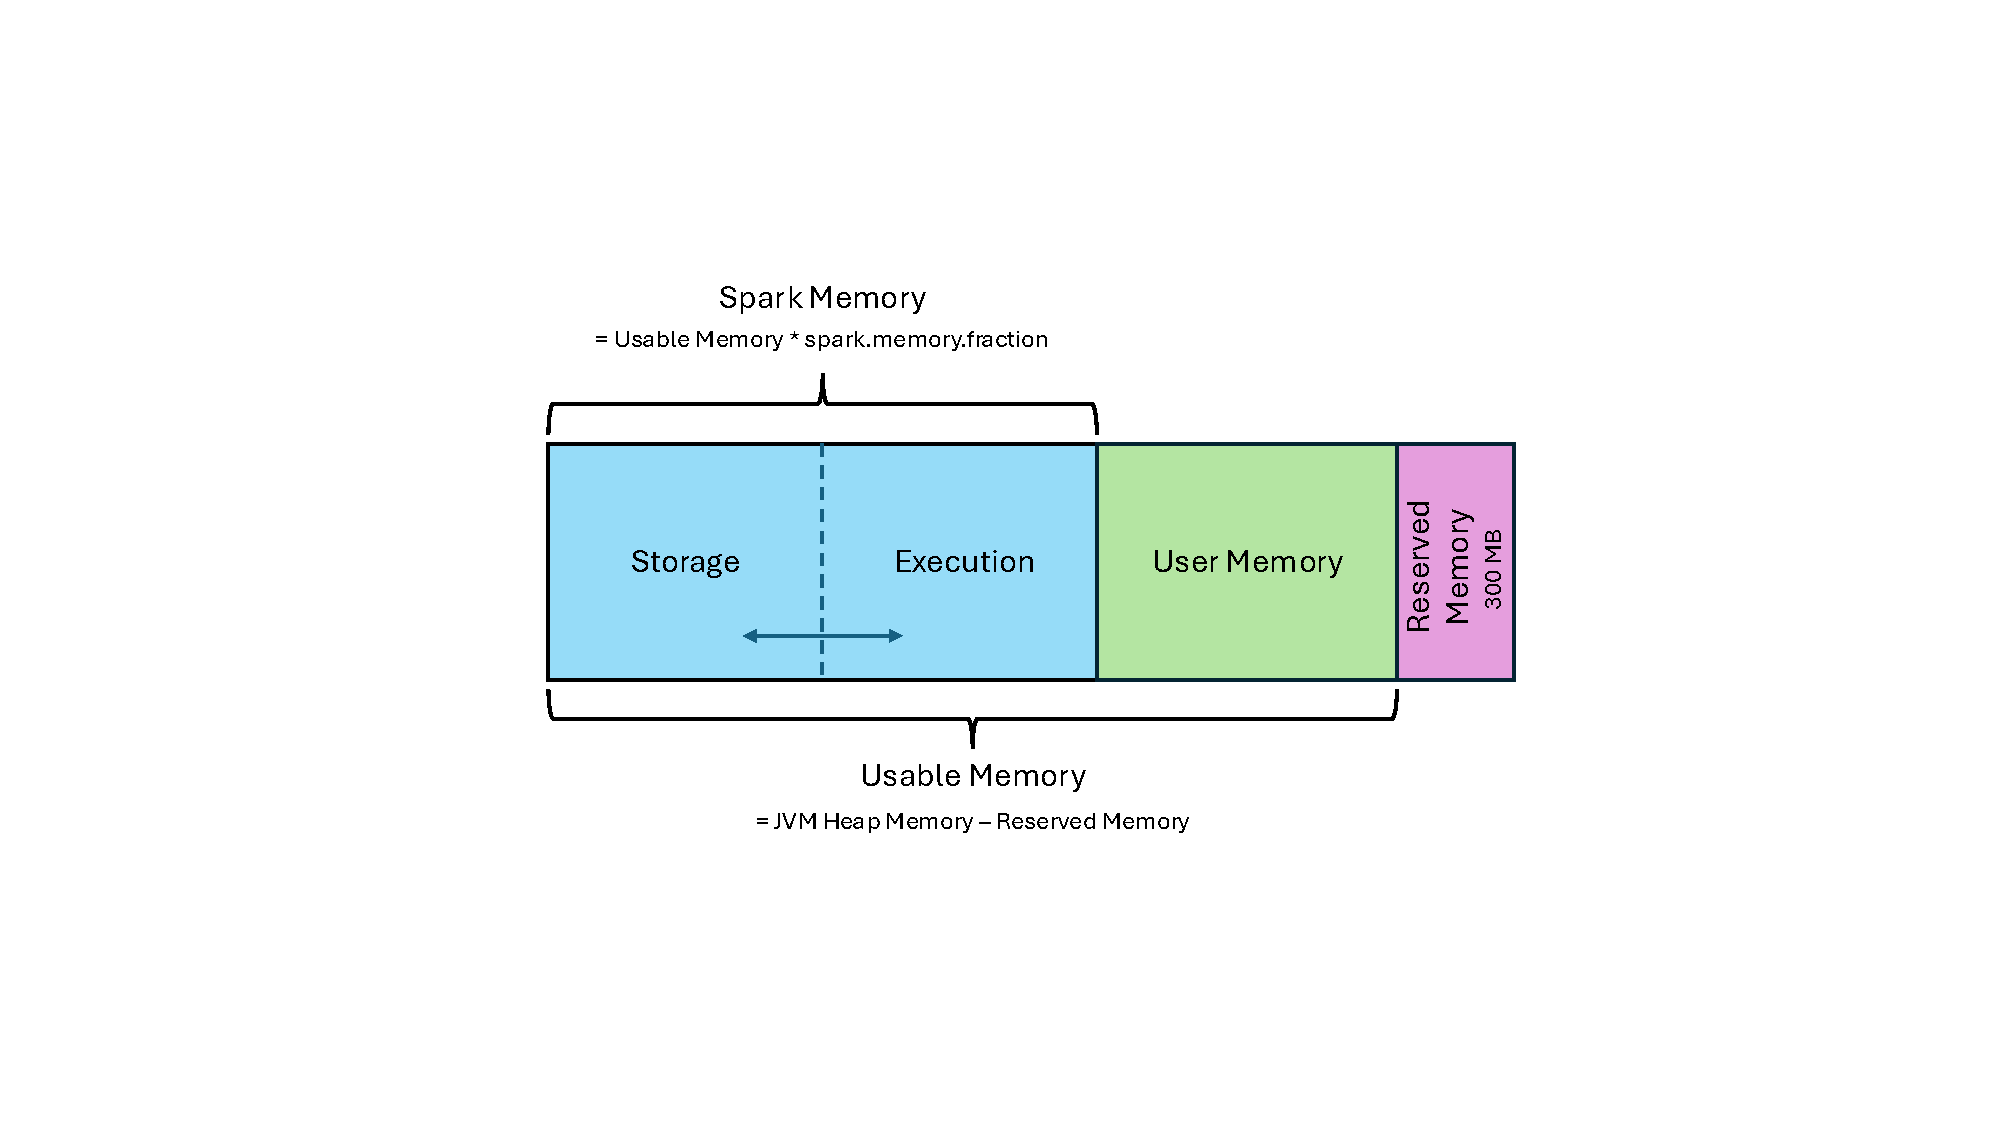
\includegraphics[width=0.7\linewidth]{images/Spark_mem_man.pdf}
    \caption{JVM Heap Memory}
    \label{fig:spark-mem-man}
\end{figure}

\textbf{Reserved Memory.} Of the total memory allocated to an executor, 300 MB are reserved for storing Spark's internal objects. This amount is constant across all executors and guarantees sufficient memory for the system \cite{apache_spark_configuration_2025}.
\textbf{Spark Unified Memory.} This section comprises the usable memory, which is divided into two subregions: \textbf{Spark Memory} and \textbf{User Memory}. The memory allocation depends on spark.memory.fraction. Typically, $0.6$ of the memory is allocated to Spark Memory and $0.4$ to User Memory. Forty percent of the user memory is used to store user data and the results of operations. Spark memory consists of execution and storage memory. Execution memory mainly stores temporary data for computations such as shuffles, joins, and aggregations, while storage memory holds cached data and broadcast variables. Furthermore, the memory allocation between the two can be configured through spark.memory.storage.fraction, where the default value is $0.5$. A special feature of Spark memory is its flexibility. Spark allows executor and storage memory to borrow from each other. This is called the dynamic occupancy mechanism. However, this feature has some limitations. Storage memory can borrow as much execution memory as needed when execution memory is idle. Execution memory, however, can only borrow up to a certain threshold called onHeapStorageSize. Storage memory only uses this part when it's not occupied by execution memory. Storage memory cannot evict execution memory and must wait until it is free. Conversely, execution memory has priority and can evict borrowed memory. In that case, cached data will be evicted until sufficient memory is released. This is because executing a task is more critical than cached data. A task can fail if execution results in an Out-of-Memory (OOM) error. Most operations, however, are executed in on-heap memory, which is subject to garbage collection (GC). Spark can move certain operations to off-heap memory to reduce GC overhead. In this case, memory is stored outside the JVM heap, enabling Spark to manage memory more efficiently. This improves performance for larger workloads, but adds a layer of complexity since Spark must handle memory allocation and deallocation. \cite{chambers_spark_2018}\cite{apache_spark_tuning_2025}. 

\subsection{Resilient Distributed Dataset}

\subsubsection{Definition and Properties of RDDs}
\subsubsection{Lineage and Fault Tolerance}
\subsubsection{Transformations vs. Actions}
\subsubsection{Caching and Persistence}
\subsubsection{Implications for Iterative Graph Algorithms}

A Resilient Distributed Dataset (RDD) is the core abstraction in Spark. An RDD is a partitioned collection of elements that is distributed across the nodes of a cluster. It is processed in parallel \cite{apache_spark_rdd_2025}. RDDs are immutable and resilient to failures due to lineage, which is a feature that records all transformations applied to the data. In the event of a node failure, lost data can be recomputed using these records. RDDs can perform two types of operations: transformations and actions. Each transformation, such as map, filter, or join, creates a new RDD. An action, such as, count, triggers execution. RDDs can be cached or persisted in memory to avoid recomputation with each iteration \cite{chambers_spark_2018}. However, since RDDs are immutable, every transformation creates a new RDD. This can easily result in high memory usage, especially when computing iterative graph algorithms, such as PageRank, where each iteration creates new RDDs for vertex properties. 



\subsection{State of the Art}
% Iteration, sampling, matrix approximation, and Monte Carlo approaches.

\subsubsection{Iteration-Based Methods}
\subsubsection{Sampling-Based Methods}
\subsubsection{Matrix Approximation Methods}
\subsubsection{Monte Carlo Methods}
\subsubsection{Trade-offs: Accuracy vs. Efficiency}

The standard PageRank method uses power iteration, which requires storing the entire graph structure in memory. The PageRank values are updated with each iteration until convergence. For large graphs, this process is computationally and memory-intensive, rendering it impractical. Therefore, approximate PageRank algorithms have been proposed for practical, large-scale analysis, which trade off accuracy for efficiency \cite{wu_efficient_2024}. The following methods have been introduced:
\textbf{Iteration methods} \cite{xie_parameterized_2023-1}\cite{anikin_efficient_2022} accelerate the standard power iteration but still operate on the whole graph structure \cite{wu_efficient_2024}. 
\textbf{Sampling-based methods} estimate PageRank values by using smaller, sampled subgraphs \cite{bar-yossef_local_2008}\cite{chen_local_2004}. Despite reducing the size of the input data, these methods cannot estimate the PageRank values for the vertices outside the sampled set \cite{wu_efficient_2024}.
\textbf{Matrix approximation methods} use a low-rank approximated transition matrix to estimate PageRank values \cite{liu_fast_2015}\cite{benczur_feasibility_2005}. 
\textbf{Monte Carlo methods} estimate PageRank values by simulating random walks on the graph. Rather than iteratively updating a full rank vector, these models simulate many random walks on the graph \cite{avrachenkov_monte_2007}. A node's value is estimated by the number of walks that end at the vertex. To achieve high accuracy, these methods require a large number of iterations \cite{wu_efficient_2024}. However, the amount of memory required for the simulation can be controlled by the number of concurrent random walkers rather than by the total number of vertices \cite{avrachenkov_monte_2007}. Given the potential memory advantages of controlling the number of random walkers, Monte Carlo methods offer a promising approach for approximating PageRank on a large scale.